\documentclass{article}
\usepackage[utf8]{inputenc}
\usepackage{graphicx}
\usepackage{hyperref}
\usepackage{subcaption}
\usepackage{amsmath}
\usepackage{amsfonts} 
%\usepackage{multirow}
%\usepackage{multicol}
\title{DPhil: Transfer of Status Literature Review}
\author{Shaan Desai }
\usepackage[parfill]{parskip}

\begin{document}

% Title page is created here
\maketitle
\bibliographystyle{abbrv}
\pagebreak
\tableofcontents
\pagebreak
\section{Introduction}

Humans have long tried to understand how the mind works. From a biological perspective, connectomics has paved a pathway to understanding how we think \cite{cowan_neural_1990}. Inspired by these ideas and the advent of computers and increased processing power, many researchers in the 50's began to ask whether the human mind can be replicated using a computer. Early work by Walter and Warren was one of the first to point out a means to build neural logic in computers that loosely resembles neurons in the brain \cite{cowan_neural_1990}. Their seminal work opened up a new door to AI research and was later proven to hold universal function approximation properties \cite{hornik_multilayer_1989}. Given neural networks are inspired by brain activity and consist of mathematical guarantees, AI researchers have focused intensely on developing them further. Arguably, they have been the most used method in the past decade having shown remarkable performance across a whole host of domains including image classification \cite{he_mask_2018}, machine translation \cite{devlin_bert_2019} and robotic manipulation \cite{toussaint_differentiable_2018}. Despite these grand successes, neural networks have numerous limitations. Firstly, they are considered 'black box' models meaning they aren't readily interpretable. Secondly, they require a significant number of data points ($>5000$ points) to learn and thirdly, they are highly sensitive to hyper-parameter tuning. Given such limitations, the physics community has been apprehensive about their adoption. However, over the past two years, significant research in \textit{scientific machine learning} has created a new road to tackle the limitations of neural networks by embedding knowledge from physics into them. This prior knowledge has been shown to make neural networks more data efficient, interpretable and stable. In this review, we canvas state-of-the-art methods that incorporate physics into deep neural networks. For each method, we summarize the key insights that drive performance and also mention possible pain points worth investigating further.



\section{Inductive Biases}

An inductive bias in machine learning is prior information used to guide model building. In simple linear regression, for example, we may assume the distribution of the noise in our data follows a Gaussian. This is a natural inductive bias because it imparts prior knowledge on the noise model of our data. In neural networks, architectures with variable depth, form and activations for example, serve as inductive biases. In essence, inductive biases allow us to encode initial assumptions about the complexity of our data.

A feedforward deep neural network naturally encodes non-linearity as a prior and arguably makes the least assumptions about the underlying data. Convolutional Neural Networks assume spatial representations can be captured. Recurrent Neural Networks assume temporal data as inputs \cite{battaglia_relational_2018}.

In what follows, we highlight some of the recent advances in inductive biases, particularly as they relate to solving problems in physics.

\subsection{Graph Neural Networks}

\begin{figure}[h]
\centering
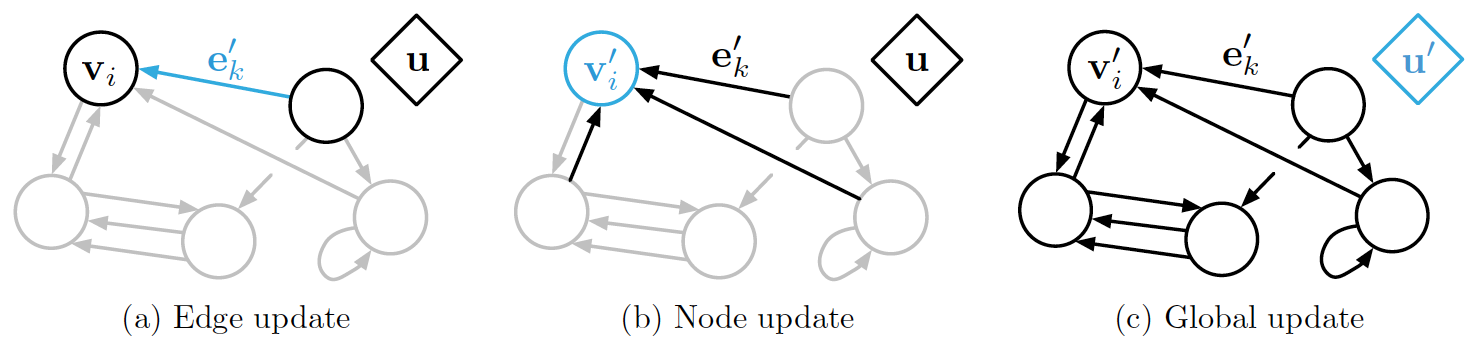
\includegraphics[width=\textwidth]{figures/1graph.png}
\caption{Graph attribute updates as presented in \cite{battaglia_relational_2018}. GNNs carry out a sequence of computations and aggregations at an attribute level to determine the next set of values.}
\label{fig:gnn}
\end{figure}
The state of a dynamic physical system can be represented by a graph $G$ consisting of vertices $V$, edges $E$ and global parameters $u$ often denoted as $G = (u,V,E)$ \cite{battaglia_relational_2018}. For example, a node ($V$) can be used to represent a particle in an N-body problem. These nodes can be used to contain the core features of the particle e.g. position, momentum, mass and particle constants. Edges ($E$) can represent forces between the particles and `Globals' ($u$) can represent constants such as air density, the gravitational constant etc. We note that graphs can be fully connected or sparse, depending on the specific use case. In representing physical systems this way, we impart structure on our data which forms an important inductive bias when learning physics \cite{battaglia_interaction_2016, battaglia_relational_2018, sanchez-gonzalez_graph_2018,seo_differentiable_2019,cranmer_learning_2019, seo_physics-aware_2020, sanchez-gonzalez_learning_2020,lamb_graph_2020,cranmer_lagrangian_2020}. Representations of this form allow us to carry out learning in multiple complex domains because such graphs impart a strong relational bias on the data. Graph Neural Networks are designed to translate graphs from one state to another. They work by computing sequential updates to node, edge and global parameters and aggregating them to define a new output graph. Graph Neural Networks are considered to impart a relational inductive bias, as convolutional networks are considered to impart a spatial bias and recurrent networks to impart a temporal bias. 

Some major applications of GNNs include:
\begin{itemize}
\item Interaction-physics based problems naturally benefit from GNNs \cite{battaglia_relational_2018}. 
\item GNNs trained to learn Hamiltonians achieve impressive results in rolling out trajectories of large N-body systems \cite{sanchez-gonzalez_hamiltonian_2019}. 
\item GNNs have shown significant promise in explaining the phase transitions of glassy materials \cite{bapst_unveiling_2020}. 
\item GNNs can learn complex fluid like systems from visual data \cite{sanchez-gonzalez_learning_2020}. 
\end{itemize}

\textbf{Bottom Line}: Inspired by this work we see two major steps in moving this research forward. Firstly, their use in physics opens up a tried-and-tested pathway to solve more complex problems particularly in accounting for material interactions. As such, we see good scope to use graph networks for large interacting systems as has been shown in \cite{sanchez-gonzalez_learning_2020}. Secondly, most systems to date have looked at graphs for classical physics, but literature from 2004 suggests graphs, inherent in their relational structure, can also capture Ising-like Hamiltonian structure \cite{rezek_operator_nodate}. In addition, although Hamiltonian Graph Networks show strong performance \cite{battaglia_relational_2018}, not much work has been done to uncover the learned relations and whether they are consistent with ground truth interactions.


\subsection{Integrative Biases}

\begin{figure}[h]
\centering
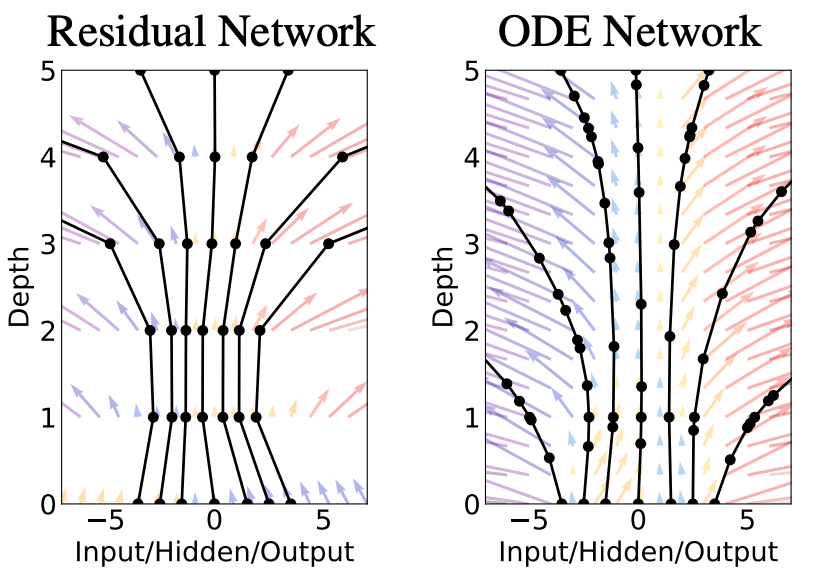
\includegraphics[width=0.8\textwidth,height=5cm]{figures/2odenet.png}
\caption{ ODE Networks \cite{chen_neural_2018} show that in the continuous time limit, residual networks look like integrated neural networks.}
\label{fig.odenet}
\end{figure}
NeuralODE brought to light a meaningful connection between residual networks and integrative steps \cite{chang_reversible_2017,chen_neural_2018}. Residual networks are able to model complex functions by sequentially transforming a hidden state. Mathematically, this might look as follows:

\begin{equation}
h_{t+1} = h_t + f_{\theta}(h_t)
\label{eqn.odedisc}
\end{equation}

where $h_t$ is a hidden layer of the network and $f_{\theta}(h_t)$ is a neural network parametrized by $\theta$ that operates on a hidden layer. By combining these discrete transformations over $t$, one can obtain more complex, non-linear functions that may be needed for downstream tasks \cite{he_deep_2015}.

If more steps are taken at shorter time intervals, in the continuous limit, equation \ref{eqn.odedisc} becomes:
\begin{equation}
\frac{dh(t)}{dt} = f(h(t),t,\theta)
\end{equation}

Using this logic, we can parametrize any differential equation as a neural network and integrate it as long as we know its initial condition and final time step evaluation. However, one of the challenges of passing a neural network output to an integrator is the fact that the integrator induces additional operations on the weights i.e. this process becomes a continuous depth neural network if the final time evaluation is large in comparison to the discrete time steps between layers. Neural ODEs via the adjoint method allow us to integrate this neural network with constant memory cost \cite{chen_neural_2018} using an ODESolver.

NeuralODE is used in numerous systems aimed at learning continuous time dynamics. In many settings a one-step integration is applied. For this, a complex ODESolver is replaced in favour of a simple explicit integrator e.g. Runge-Kutta 4. There are indeed settings where a multi-step integration is used, such as in \cite{zhong_symplectic_2019} and in \cite{saemundsson_variational_2019} for which continuous depth networks cause severe memory issues if NeuralODE is not used.

Despite their success, the work in \cite{dupont_augmented_2019} identifies the instability of using the adjoint method to compute continuous depth networks and propose a method to resolve this issue. 

\textbf{Bottom Line}: Extensions of this work have been adopted across numerous methods we are about to discuss. Future work in this direction should look at identifying the right integrator of choice and establishing whether neural integrators can circumvent the need for an ODESolver.

\subsection{Physics priors}

Broadly, the intersection of physics and AI falls into one of two domains, physics for AI or AI for physics. The former uses techniques from physics to develop and improve learning algorithms in general. The latter uses existing learning approaches (with adaptations) to performance inference over physical systems, for example ML for materials \cite{rupp_fast_2012,smith_ani-1_2017}. In this review, we focus our attention on the latter.

Physicists have long been interested in using learning tools to predict physics based systems. Some of these include predicting magnetic properties of 2-D materials \cite{rhone_data-driven_2018}, predicting the time evolution of N-body systems \cite{battaglia_relational_2018} and even using AI to understand phase transitions \cite{bapst_unveiling_2020}. However, numerous challenges still remain in terms of 1. data-efficient learning, 2. reducing computational cost, 3. improving predictive accuracy and 4. learning better representations of the underlying physical process. Researchers have identified methods to address these challenges, but arguably the most promising hinges on physics-informed priors embedded in learning. It has been shown that models enriched with physically-informed priors i.e. models which consist of some knowledge about the physical system apriori, significantly outperform traditional methods in terms of data-efficiency and predictive accuracy. This has sparked a sharp interest in building both task-specific and general physics priors to improve learning. In this section, we summarize some of the core developments over time in physics informed inductive biases. 

\subsection{Gradient Learning}

Although most modern methods cite gradient learning by Witkoskie \cite{witkoskie_neural_2005} as one of the earliest efforts designed to improve learning of physics in neural networks, we actually find that a more sophisticate approach was developed prior to this effort.

In 1996, James Howse \cite{howse_gradient_1996} presented a paper that highlights an approach to identify dynamical systems. The paper introduces a model inspired by defining a generalized functional form for dynamical systems. Using a potential $V(x)$ the authors show that we can partition an n-dimensional phase space into two components. The first space is normal to a level surface $V(x)=k$, and the second is tangent to $V(x)=k$. Systems that always move downhill are gradient like systems: $ \dot{x} = - P(x)\nabla_{x} V(x) $. Systems that remain at constant potential are Hamiltonian like: $\dot{x} = Q(x)\nabla_x V(x)$. The paper shows that by casting a dynamic problem into these two components, one can learn the coefficients of the dynamical system. 

In addition, the notion of embedding physically-informed inductive biases in neural networks can be found in numerous early work aimed at modelling materials \cite{witkoskie_neural_2005, pukrittayakamee_simultaneous_2009, smith_ani-1_2017, rupp_fast_2012, yao_tensormol-01_2018}. For example, early efforts by Witkoskie and Doren \cite{witkoskie_neural_2005} demonstrate that in contrast to directly learning a potential energy surface, the inclusion of gradient learning can drive a network to accurately model the forces. By gradient learning we mean that instead of a state vector being defined as $x$ over which we want to optimize, our state vector becomes $[x,\dot{x}]$. This addition means that we can supplement the learning process with additional information and hence improve the learnt potential surface. The fundamental idea being that if we have access to supplemental data such as the gradients, but fewer data points, we might actually learn a surface with higher accuracy than if we had many data points with no gradient information. 

\textbf{Bottom Line}: This result inspires us to look more closely at combining inductive biases. Namely, by adding well known priors together, we may make learning data-efficient and more accurate. In addition, we might want to look more closely at the results in \cite{howse_gradient_1996} to see if we can develop a more generalizable approach to learning dynamics.

\subsection{PINNs: Physics Informed Neural Networks}

PINNs are one of the first methods to use the backpropagation technique from neural networks to actually compute the gradients of a function with respect to the inputs of that given function. The core idea in PINNs is to solve the following equation:

\begin{equation}
 u_t + \mathcal{N}[u] = f = 0
\end{equation}

where $u(t,x)$ is a function that depends on time $t$ and state-vector $x$ and where $\mathcal{N}$ is a non-linear differential operator. $u(t,x)$ denotes the latent hidden solution. To solve this equation, when only the initial conditions of $u$ and specific collocation points are provided, PINNs compute $u(t,x)$ with a neural network. Using backpropagation, they then compute partial derivatives with respect to the input variables $t,x$. The final results can thus be stored in $f$. A simple L2 loss to minimize the predicted $u_{pred}$ vs. the ground truth $u_{gt}$ (for initial and boundary conditions) coupled with a penalization of the function $f$ (since it should be zero) at specific collocation points results in PINNs.

PINNs are used for both data-driven solutions and data-driven discovery. In other words, PINNs can be used to identify a system's governing equations, or given a set of equations, be used to continuously solve the system given an initial condition and points of evaluation.

One limitation to this approach is the need to know the functional form of $\mathcal{N}$. However, the authors of PINNs also developed deep hidden physics models \cite{raissi_physics-informed_2019} that are designed to learn the functional form without any prior knowledge of the function $\mathcal{N}$. The idea behind these deep hidden physics models is to compute $u$ and then compute up to the  k-th order derivatives of $u$. Using a regressive search, one can then identify the components that make up the underlying equation. 

\textbf{Bottom Line}: PINNs are a versatile method that use backpropagation to compute both the loss term and the gradients of the function $u$ w.r.t its inputs. 

\subsection{Energy Conserving Networks}

As the section title suggest, energy conserving networks aim at conserving the energy of a given trajectory. The section looks carefully at methods that attempt to learn the Hamiltonian or Langrangian of a system.

\subsubsection{Hamiltonian Neural Networks}
\label{HNN}
\begin{figure}[h]
\centering
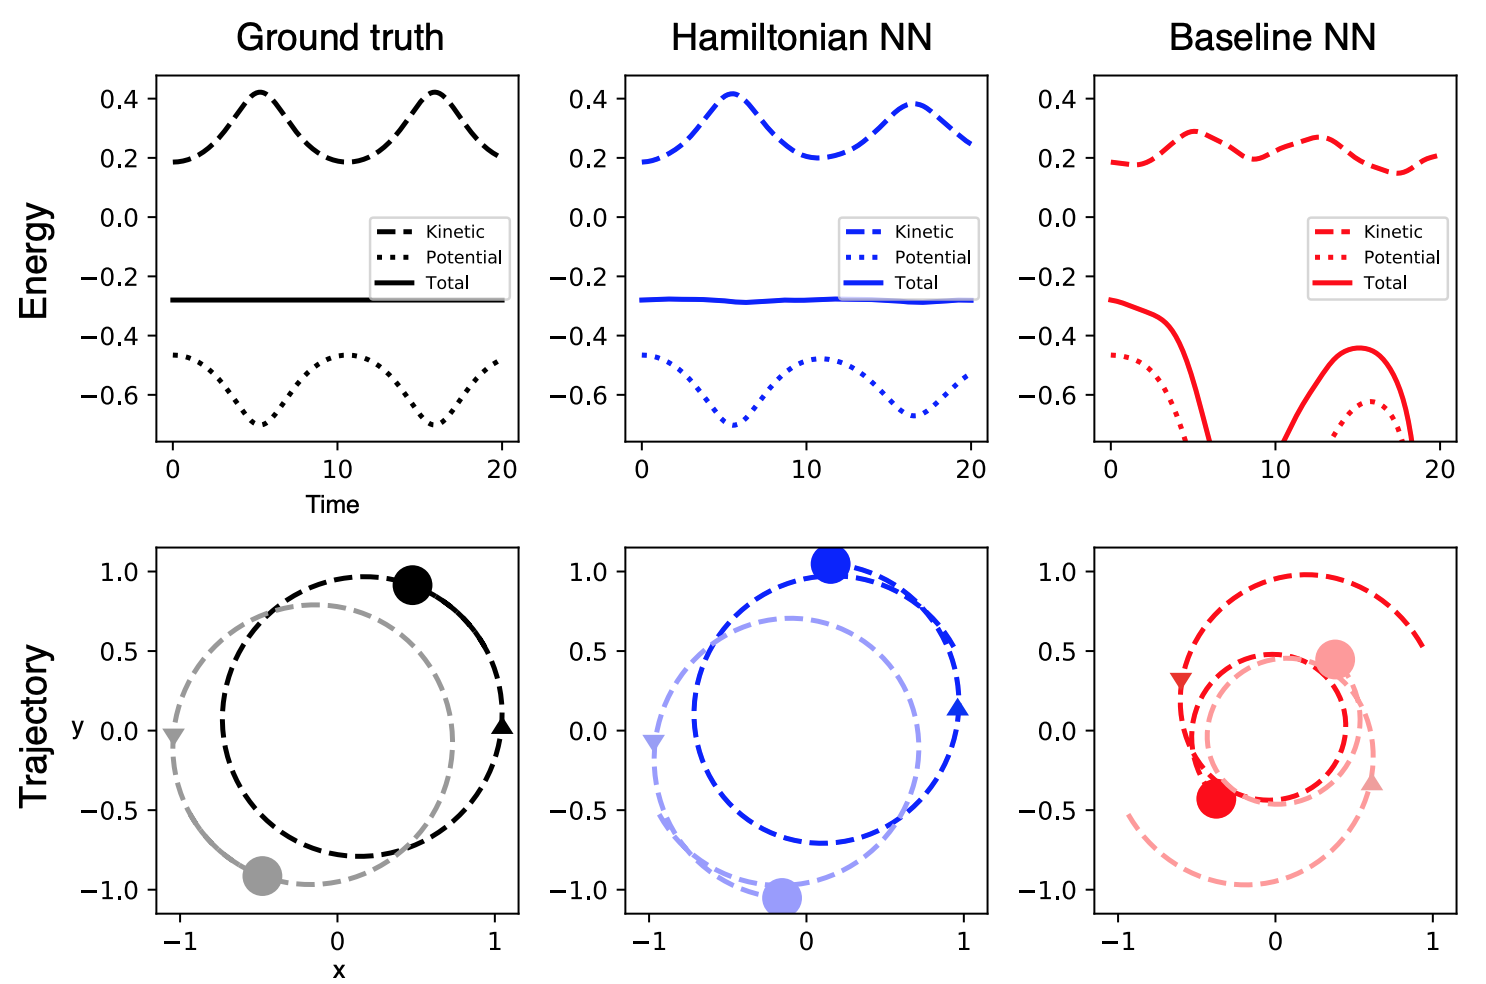
\includegraphics[width=\textwidth]{figures/3hnn.png}
\caption{Trajectories of a 2-body system as predicted in \cite{greydanus_hamiltonian_2019}.}
\end{figure}

The work in \cite{greydanus_hamiltonian_2019} demonstrates that dynamic predictions through time can be improved using Hamiltonian Neural Networks (HNNs), which endow models with a Hamiltonian constraint. The Hamiltonian is an important representation of a dynamical system because it is one of two approaches that generalizes classical mechanics. The Hamiltonian $\mathcal{H}$ is a scalar function of position $\mathbf{q} = (q_1,q_2,....,q_M)$ and momentum $\mathbf{p} = (p_1,p_2,....,p_M)$. In representing physical systems with a Hamiltonian, one can simply extract the time derivatives of the inputs by differentiating the Hamiltonian with respect to its inputs (see Eqn. \ref{eqn.hamiltonian}.)
\begin{equation}
\frac{\mathrm{d}\mathbf{q}}{\mathrm{d}t} = \frac{\partial \mathcal{H}}{\partial \mathbf{p}}, ~~~
\frac{\mathrm{d}\mathbf{p}}{\mathrm{d}t} = -\frac{\partial \mathcal{H}}{\partial \mathbf{q}}
\label{eqn.hamiltonian}
\end{equation}
As a consequence, it is noted in \cite{greydanus_hamiltonian_2019} that by accurately learning a Hamiltonian, the system's dynamics can be naturally extracted through backpropagation, similar to \cite{raissi_physics-informed_2019}. This information allows us to build two 1st-order differential equations which can be used to update the state space, $(\mathbf{q},\mathbf{p})$. Equation \ref{eqn.action_int} shows this integral, in which we define the symplectic gradient $\mathbf{S}  = \left [ \frac{\partial \mathcal{H}}{\partial \mathbf{p}},-\frac{\partial \mathcal{H}}{\partial \mathbf{q}} \right ] $:
\begin{equation}
(\mathbf{q},\mathbf{p})_{t+1} = (\mathbf{q},\mathbf{p})_t + \int_t^{t+1} \mathbf{S}(\mathbf{q},\mathbf{p}) \mathrm{d}t
\label{eqn.action_int}
\end{equation}
%However, this is not the only benefit in learning a Hamiltonian. Another key attribute of the Hamiltonian is that the vector field $\mathbf{S}$ is a symplectic gradient meaning $\mathcal{H}$ remains constant as long as state vectors are integrated along $\mathbf{S}$. This result links the Hamiltonian with the total energy of the system $\mathcal{H}(\mathbf{q},\mathbf{p}) = E_{tot}$. 
It can be shown that the Hamiltonian in many systems also represents the total energy of the system. Therefore, the Hamiltonian is a powerful inductive bias that can be utilised to evolve a physical state while maintaining energy conservation.

As we will discuss later, HNNs are great at learning in low-dimensional settings for a few integration steps. However, scaling this network to more challenging problems proves difficult. Fortunately, many alternatives have been proposed. 

\textbf{Bottom Line}: One limitation we hope to investigate further in this domain is adding an energy penalization term between the predicted and ground truth energies to make learning more data-efficient. Our preliminary experiments find that penalizing the loss function with an energy term actually hurts the learning process indicating instability issues linked to HNNs. 

\subsubsection{Variational Integrator Networks}

Lagrangian mechanics offers an alternative to the Hamiltonian in generalizing a dynamical system. Rather than position and momentum (canonical coordinates) defining the state space, Lagrangian mechanics is defined using a generalized coordinate state space $(\mathbf{q},\dot{\mathbf{q}})$. This is particularly useful in physical settings where the description and measurement of generalized coordinates may be easier to work with than canonical coordinates \cite{marsden_discrete_2001}. Given these coordinates, Joseph-Louis Lagrange showed that a scalar value $\mathcal{A}$, referred to as the action, can be defined as the integral of a Lagrangian, $\mathcal{L}(\mathbf{q},\dot{\mathbf{q}})$:
\begin{equation}
\mathcal{A} = \int_{t}^{t+1} \mathcal{L}(\mathbf{q},\dot{\mathbf{q}}) \mathrm{d}t
\label{eqn.action_integral}
\end{equation}
The integral can be thought as inducing multiple paths between points in state space i.e. multiple walks in the domain of $(\mathbf{q},\mathbf{\dot{q}})$. However, only one path is a stationary state of the action integral. This state lets us move from $t \rightarrow t+1$ with minimal energy. It can be shown, through variational calculus, that this stationary state must satisfy the Euler-Lagrange equation:
\begin{equation}
\frac{\mathrm{d} }{\mathrm{d}t} \left ( \frac{\partial \mathcal{L}}{\partial \dot{\mathbf{q}}} \right )= \frac{\partial \mathcal{L}}{\partial \mathbf{q}}
\label{eqn.euler_lagrange}
\end{equation}
Although complex in form, the action integral and the Euler-Lagrange equations can be discretized and collectively form the basis for variational integrators. The work in \cite{saemundsson_variational_2019} shows that, by adopting this approach, one can develop VINs which make network learning in noisy data-settings more robust. Similar to Hamiltonians, Lagrangians in classical mechanics are also connected to the kinetic energy $\mathcal{T}$ and potential energy $\mathcal{V}$ via:
\begin{equation}
\mathcal{L} = \mathcal{T}(\mathbf{q},\mathbf{\dot{q}}) - \mathcal{V} (\mathbf{q},\mathbf{\dot{q}})
\end{equation}
Furthermore, Variational Integrators are symplectic and momentum conserving \cite{lew_overview_nodate}.

\textbf{Bottom Line}: The paper introduces the importance of symplectic integrators but does not discuss how to improve accuracy and scale up to higher dimensions. It is with this in mind that VIGNs was borne.

\subsubsection{Deep Lagrangian Network}

DeLAN net is the first network to use a Lagrangian embedded in a neural network to learn the dynamics of a system \cite{lutter_deep_2019}. 

The paper defines the Langrangian $\mathcal{L} (q,\dot{q})$ and Euler-Lagrange equations to be:
\begin{equation} 
\mathcal{L} = T - V
\end{equation}
and

\begin{equation}
\frac{d}{dt}\frac{\partial L}{\partial \dot{q}} - \frac{\partial L}{\partial q} = \tau
\end{equation}

where $\tau$ represents generalized forces, $T$ is kinetic energy and $V$ is potential energy.

If we are dealing with a rigid body then: $ T = \dot{q}^{\mathrm{T}} M(q) \dot{q} $ where M is the inertia matrix. Replacing this equation in the Euler-Lagrange equation results in:

\begin{equation}
 \frac{d}{dt} (M(q)\dot{q}) - \frac{\partial V}{\partial q} = 0; 
~~~
M(q)\ddot{q} = \dot{M(q)} \dot{q} + \frac{\partial V}{\partial q} 
\end{equation}

To obtain $\ddot{q}$, the method proposes computing $M$, $\dot{M}$ and $\frac{\partial V}{\partial q}$ separately and then combining them.  

\textbf{Bottom Line}: As a result of this framing, DeLAN net uses multiple network heads to compute individual components of the equation before combining them. \cite{cranmer_lagrangian_2020} show that it is indeed possible to circumvent this problem. The important result here is that DeLAN can learn individual representations. If the non-conservative forces can be distinguished e.g. damping vs forcing, then DeLAN could be used to learn individual damping/driving forces from data which could be used on other systems. 



%\subsubsection{Deep Energy Network}
%
%A new method is introduced to tackle the challenge of learning energy conserving physics more broadly. The method claims to be more general as it can learn from PDEs as well as ODEs, and it avoids discretisation errors that arise from using Runge-Kutta integrators. The method does this by a) introducing a general formalism which highlights how the rate of change of states can be cast into a matrix $G$ times the gradient of a Hamiltonian $\nabla H$ and b) by discretising the gradient of the Hamiltonian with a frechet derivative. 
%\begin{equation}
% \dot{u} = G\nabla H
%\end{equation}
% 
%The main benefit is that it can solve a broader class of problems compared to current solutions in the field e.g.
%\begin{itemize}
%\item{Friction systems (ODE and PDE)}
%\item{Discrete PDEs (PDE)}
%\item{Maintains energy and mass conservation via discretisation which preserves the geometric structure (a.k.a volume preservation)}
%\end{itemize}
%
%The main results of the paper indicate Good form for discrete auto differentiation
%Great PDE dataset motivations
%Can extend research to identify discrete PDEs


\subsubsection{Unsupervised Learning of Lagrangian Dynamics}

In \cite{zhong_unsupervised_2020}, the authors show that the full Lagrangian dynamics can be learned from visual data. The paper introduces a co-ordinate aware VAE to encode the latent space. Using the encoded latent space, a Lagrangian is learnt so that the time derivatives of the latent space can be extracted and used to integrate the latent space. The paper shows that the motion of a pendulum can be learnt from visual data. More importantly, via energy shaping, the pendulum can be constrained into a state-space $q*$ of choice.

\textbf{Bottom Line}: This result is quite powerful because it empirically proves that a controlled Lagrangian system can be learned from visual data. This inspires us to ask the question of whether a chaotic system such as heinon-heiles or the double-pendulum can be learned from visual data.

\subsubsection{Lagrangian Neural Networks}

The main premise of LNNs \cite{cranmer_lagrangian_2020} is to tackle the problem of dealing with canonical coordinate spaces. Many datasets do not usually consist of canonical position and momentum, rather they use generalized coordinates. As such, LNNs aim to address learning from generalized coordinates. In addition, they provide a more general framework than DeLANs which were designed to work well with continuous control applications. The unique innovation that LNNs introduce over other methods is that they do not assume any form for the Lagrangian. As such, they vectorized the Euler-Lagrange equation:

\begin{equation}
\frac{d}{dt} \nabla_{\dot{q}} \mathcal{L} = \nabla_q \mathcal{L}
\label{eqn.lnn1}
\end{equation}

Then, using the chain rule to expand the time derivative by allowing $\nabla_{\dot{q}}\mathcal{L}$ to be a function of $q$ and $\dot{q}$, they obtain:

\begin{equation}
(\nabla_{\dot{q}}\nabla_{\dot{q}}^T \mathcal{L}) \ddot{q} + (\nabla_q \nabla_{\dot{q}}^T \mathcal{L})\dot{q} = \nabla_q \mathcal{L}
\end{equation}

Using matrix inversion, one can obtain $\ddot{q}$. 

\textbf{Bottom Line}: The paper shows promising results on the double pendulum, relativistic particle in a uniform potential and on the wave equation. Upon inspection of the training scheme for the highly sensitive double pendulum, we do find that training times and data points are quite large, creating a space to find a more optimal learning scheme.

\subsubsection{Modeling System Dynamics with PINNs on Lagrangian Mechanics}

Unlike LNNs, this paper introduces a functional form for the Lagrangian. The Lagrangian in this paper \cite{roehrl_modeling_2020} is assumed to be $L = T -V$. In addition, the authors introduce non-conservative forces and the final form is:

$$ M(q) \ddot{q} + C(q,\dot{q})\dot{q} + G(q) = Q^{ncons} $$

The approach taken by this paper is to feed in the respective components e.g. $q$,$\dot{q}$ into separate neural network heads designed to predict one of $M$, $C$ and $G$. Using this technique, $\ddot{q}$ is backed out and then fed to a RK-4 integrator. In other words, the approach is a simplified version of DeLANs.

\textbf{Bottom Line}: The approach is tethered to a more traditional way of using NNs for predictions and is one of the reasons why model performance is not as good as it can be if backpropagation was used to compute the second derivative of q. In addition, the wrong choice of integrator is a bottleneck for long range predictions in this setting.

\subsection{Symplectic Networks}

Many researchers have identified that embedding integrators into the learning process of dynamic systems alleviates the need for the derivatives $[\dot{q},\dot{p}]$ of the state vector $[q,p]$. That is, with an integrator embedded, the state-vector is enough to compute the dynamics. However, as \cite{zhu_deep_2020} and a number of other researchers highlight, the choice of integrator can play a significant role in long range predictions. In principle, integrators that preserve symplecticity show significantly better long range results because they enforce phase-space volume conservation.

\begin{figure}
\centering
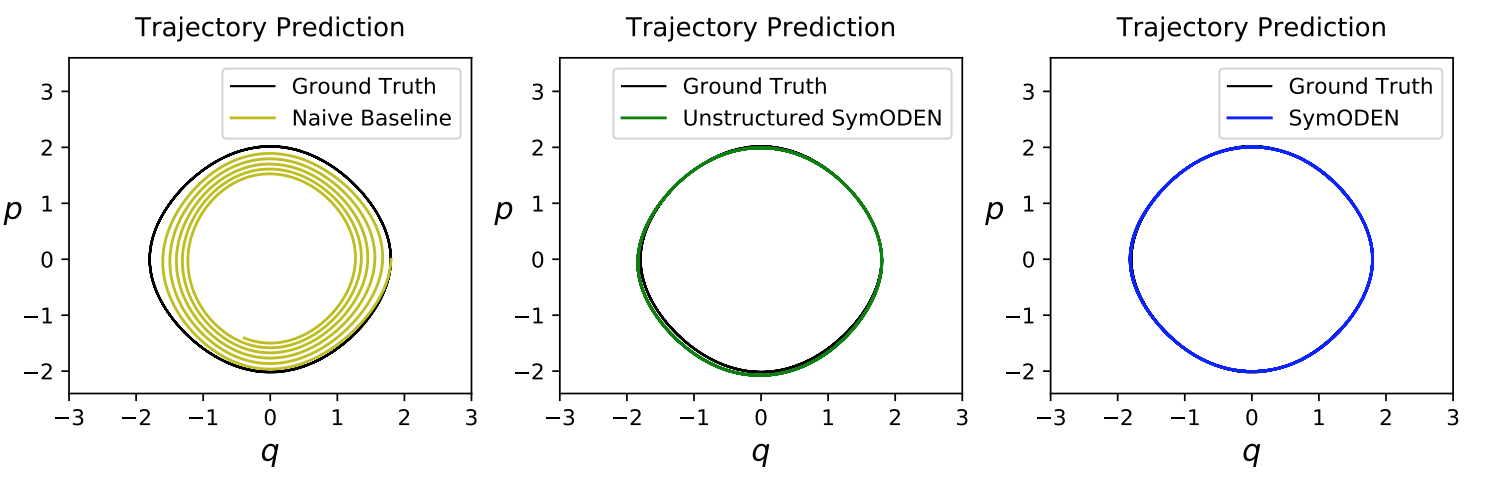
\includegraphics[width=\textwidth]{figures/4sympnet.png}
\caption{Symplectic Integrators from \cite{zhong_symplectic_2019} illustrate their improved capacity over non-symplectic integrators at predicting long range trajectories that preserve phase-space volume.}
\end{figure}

\subsubsection{Symplectic ODE Net}

Symp-ODEN \cite{zhong_symplectic_2019} extends HNNs into the control domain. If external control is affine and influences the change in generalized momenta then the state-space derivatives can be written as:

\begin{equation}
\begin{bmatrix}
\dot{q} \\
\dot{p}
\end{bmatrix}
= 
\begin{bmatrix}
\frac{\partial H}{\partial p} \\
-\frac{\partial H}{\partial q}
\end{bmatrix}
+
\begin{bmatrix}
0 \\
g(q)
\end{bmatrix} u
\end{equation}

where $g(q)u$ represents a control variable. If rank($g(q$)) is rank($q$) the system is fully actuated \cite{zhong_symplectic_2019}. For such systems, a controller $u = \beta(q) +v(p) $ can be designed to change the potential energy landscape so as to force a system toward a specific configuration.

%If the Hamiltonian is a Newtonian then the authors show:
%
%$$ \beta(q) = g^T (gg^T)^{-1} (\partial V/\partial q - \partial V_d/\partial q) $$

Arguably this is the first paper to think extensively about the bottlenecks presented in HNNs including control, energy shaping and symplecticity. 



\subsubsection{Symplectic Recurrent Neural Network}

Symplectic RNN \cite{chen_symplectic_2020} makes two major contributions to the physics neural network space. Firstly, they take \nameref{HNN} and convert the integration scheme from euler to a leapfrog. Secondly, they adopt a NeuralODE style integrator to integrate across multiple timesteps from an initial condition. However, the results in this paper overlap greatly with Symp-ODEN. 

\subsubsection{Deep Hamiltonian Networks based on symplectic integrators}

This paper \cite{zhu_deep_2020} reviews the integrator of choice for HNNs. One of its primary objectives is to establish the difference in performance between using a symplectic vs non-symplectic integrator from a theoretical perspective. Quite evidently, using a symplectic integrator allows us to conserve the phase-space volume of the system - a crucial component in preserving energy. Their results reiterate the need for symplectic integrators when dealing with Hamiltonian-like systems.

\subsubsection{SympNets}

A brand new class of methods is proposed in \cite{jin_sympnets_2020}. It avoids the need for a separable Hamiltonian and more importantly, is designed to eliminate the need for backpropagating the Hamiltonian with respect to the input. In this framework, a sequence of symplectic maps are used to transform the input into the output. The symplectic map can be split into an upper triangular matrix and lower triangular matrix with diagonals set to 1. Non-diagonal terms are parametrized by a neural network and by stacking a range of symplectic maps together, one can learn dynamics better. In fact, the results show that by doing this, the learned trajectory is significantly more accurate than HNNs with symplectic integrators.

\textbf{Bottom Line}: The introduction of SympNets takes us in a direction tangential to the concept of backpropagating a function with respect to its input. This might be more flexible in the long run since it avoids complicating backpropagations. 

\subsection{Gaussian-Based Physics Networks}
\subsubsection{Learning Constrained Dynamics with Gauss' Principle adhering Gaussian Processes}

The work of \cite{geist_learning_2020} introduces a Gaussian Process (GP) model that utilises mechanical constraints as prior knowledge for learning system dynamics. The GP is constrained to satisfy Gauss' Principle. Using the Udwadia Kalaba equation, the acceleration of a particle can be disentangled into an unconstrained acceleration, an ideal constraint and a non-ideal constraint. Using this knowledge, one can feed this structural form into the mean of a Gaussian Process regression. The process can be used to set priors on unknown parameters linked to the constraints.

The proposal is important because it tackles constraint optimisation of physics based networks using GPs which can give us explicit uncertainty bounds on our learned trajectories.


\subsubsection{Bayesian Hidden Physics Models}

In \cite{atkinson_bayesian_2020}, the author presents a novel approach to tackle learning from noisy data. The paper is arguably the first method to combine Gaussian Processes with physics informed neural networks in a unified manner.

\textit{Problem Statement}

Given, $x$, $t$ and some initial conditions, learn the governing equation $\mathcal{N}$ of a dynamic system that obeys:

$$ u_t + \mathcal{N}[u] = 0 $$

The learning takes place in 3 stages. The first is, given inputs $x$ and $t$, compute $u(x,t)$ using a neural network. The loss of this predicted term is computed using a log likelihood s.t.:

$$ L_i^u = \log p(D_i^u|\theta_i^u) = \sum_{j=1}^{n_{st}} \log p(\hat{u}_j^{i} | u(x_j,t_j;\theta_i) $$

where $D$ is the dataset, $\theta_i$ are the network parameters and $\hat{u}$ is the ground truth function. $i = 1,...,N$ for separate parameters $\theta_i$. $n_{st}$ is the number of samples we have e.g. $ D_i = {x_j,t_j,\hat{u}_j}_{j=1}^{n_{st}} $.

Then, using the computed $u$, define a non-linear function $f(v)$ of the derivatives of $u$ where $v = (u_t,u_x,u_xx,...)$. The purpose of doing this is for data-driven discovery. By placing a prior on $f(v)$, we can figure out the right combination of partial derivatives needed to satisfy $\frac{\partial u}{\partial t} = f(v) $. The prior on this function is assumed to be Gaussian and is of the form:

$$ L^f = p(\hat{u_t}|V) = \mathcal{N} (\hat{u}_t|\mu(V),K_f +\sigma_f^2 I) $$

where $K_f$ is an exponential quadratic function and $\sigma_f^2$ is the variance of the Gaussian likelihood.
The paper opts to use a variational approximation to $f$ since there is a large amount of data that passes through the root.

The main breakthrough of using this approach is uncertainty quantification of the learned operators and function $f(v)$ that describes the differential equation as well as the ability to inspect convergence in v-space that illustrates data coverage and our uncertainties as we move away from these training points.

\subsection{Data Driven Model Discovery}


\subsubsection{Discovering Physical Concepts with Neural Networks}

Although this review has looked closely at embedding physical laws into neural networks, some approaches such as \cite{iten_discovering_2020} take on a different approach of not assuming any prior. In other words, the paper sets the \textit{scientific process} as the prior. By feeding inputs into an encoder to learn a representation and then querying this representation before decoding, the experimental process of learning laws is designed to become a part of the network.

The only caveat to this modelling is the use of disentangled VAEs that are designed to produce orthogonal representations. The assumption here being that every new variable added to the representation should be independent and alter the output landscape separately i.e. the variables should span the output space.

Results illustrate that such a system can learn accurate latent representations necessary to evolve the time dynamics of a system, including conservation laws. The network also learns how to switch co-ordinate systems.

This presents an alternative view to learning physical systems. Motivated by this result, one can easily draw a comparison across methods to illustrate how much more data/time is needed to establish the right representation in comparison to methods naturally designed to embed physical laws. 

\subsubsection{Discovering Governing equations from data by sparse identification of nonlinear dynamical systems}

The proposed method in \cite{brunton_discovering_2016} tackles learning the governing equations of a physical system by inspecting the sparsity of a function $f$ that satisfies:
 
 $$ \frac{dx}{dt} = f(x(t)) $$
 
For most systems, the paper notes that only a small group of derivatives of $x$ are relevant to compute $f$. 
 
The method first computes higher order polynomials of the inputs and then uses sparse regression to select the parameters. 
 
This approach of `selecting' from a bag of potential functions has been explored extensively in determining governing equations. However, the method relies on having to explicitly build a large matrix of permutations. 

\subsubsection{Symbolic Pregression}

Symbolic pregression combines the approach of discovering relevant coefficients with that of Hamiltonian Neural Networks to build an unsupervised framework for discovery of differential equations \cite{udrescu_symbolic_2020}. The paper still does not reveal the functional form of the underlying constraint but the results look deeply promising in dealing with visual data. Indeed they do show that it is possible to learn a number of equations from data, however, they do mention issues linked to identifiability and the need to constrain the learnt representations to ensure convergence.

\subsection{Physics Informed Generative Adversarial Networks}

Generative Adversarial Networks (GANs) have been shown to emulate complex physical concepts such as turbulent flows. In addition, by embedding physical constraints into the generator, GANs can be used to sample deterministic physical constraints. In \cite{yang_enforcing_2019}, the authors define a general physical constraints s.t.:

$$ H[u] \leq 0$$

where $H$ is a differential operator on a state $u$. Then, by adding this constraint to the generator, we get:

$$V_C(D,G) = V(D,G) + \lambda C_{phys} $$ where:

$$ C_{phys} = \mathbb{E}_{Z} (\max(H(G(Z)),0))$$

where $V(D,G)$ is the generator loss in a classical GAN. The authors show that such a system can be used to generate samples given specific deterministic constraints e.g. generating samples of  circles given a specific radii. However, they also show that approximate samples can be drawn for which constraints might be inequalities. 

Extending this work to build physics informed images might be particularly useful in animation and in physical system modelling.

\subsection{Physics Informed Neural Network Applications}

\subsubsection{Chaos}

Using \nameref{HNN}, \cite{choudhary_physics_2019} shows that it is possible to predict the trajectory of a chaotic heinon-heiles system. In addition, they are able to predict trajectories of billiard balls under complex potential functions. The authors of \cite{cranmer_lagrangian_2020} also show that the double pendulum system can be learned from data but their approach shows significant practical limitations relating to the complexity of the model used.

\textbf{Bottom Line}: Our preliminary idea was to see if HNNs can be used to learn the dynamics of a double pendulum. However, our  results show that high energy chaotic systems are quite difficult to learn. However, this line of work can establish new ways of developing neural networks that are more sensitive to their inputs. 


\subsubsection{Materials}

In numerous papers, \cite{rupp_fast_2012,witkoskie_neural_2005,pukrittayakamee_simultaneous_2009,smith_ani-1_2017,yao_tensormol-01_2018} the use of physics priors has been used to model materials. Some have taken a more traditional ML approach to predict materials properties such as \cite{rupp_fast_2012}, while others have looked at using deep networks such as \cite{wang_machine_2019} in which convolutional networks are used to extract meaningful Hamiltonian representations of magnetic materials.


\subsection{Causality}

Bayesian networks are probabilistic graphical models that can represent conditional dependencies using a Directed Acyclic Graph (DAG). The main logic behind these methods is that a probabilistic approach to determining a marginal distribution can be linked to a graph structure if certain conditional dependencies are met. 

Learning DAGs from data is an NP-hard problem, but the NOTEARS algorithm \cite{zheng_dags_2018} presents a way to tackle this combinatorial search by converting the problem into a continuous optimization problem. The main contribution of the paper is a penalization of the weight matrix so that it is acyclic. From studies of graphs we know that the n'th power of an adjacency matrix gives us the lengths of walk $k$ between two nodes. As such, all we need to do is enforce that all the diagonals of the powers of the adjacency matrices are set to zero. 

In other words:

$$ tr(I-B)^{-1} = d $$

must be satisfied where $B$ is an adjacency matrix and d is the number of columns/rows in $B$. Embedding this into the learning process is imparting an inductive bias on learning. 

It was with this in mind that DYNOTEARS \cite{pamfil_dynotears_2020} were able to extend the work into the temporal setting and learn dynamic bayesian networks. In principle, by adding an additional weight matrix to learning and penalizing it in the same way that NOTEARS does.

Furthermore, it has been shown that the NOTEARS constraint can be embedded in graph neural networks \cite{lachapelle_gradient-based_2020,yu_dag-gnn_nodate}.


\section{Conclusion}

This literature review has explored state-of-the-art deep networks designed to learn physical systems from data. While some methods focus on energy conservation, others look to discover the underlying equations of motion. In all these settings, the use of physically informed inductive biases plays a crucial role in the learning process. With this in mind, we see numerous pathways to extending the existing literature, with emphasis on the need for better applications, improved generalizability from visual data and a focus on quantifying uncertainty. Needless to say, we are excited by the advances made in the field and see scope to extend inductive biases from other domains into neural networks.

%\section{Notes}
%
%A section to document some of my learnings over time.
%
%\subsection{GANs for Physics (Oct '19 - Jan '20)}
%
%\subsubsection*{Preliminary Ideas}
%
%Can generative networks capture the laws of physics?
%
%\begin{enumerate}
%\item Generative networks are able to learn complex mappings from data to latent spaces
%\item Often, these latent spaces are able to perfectly generate the original data which might indicate that the fundamental laws of physics are being captured by the network
%\item This leads us to the question - can we use a generative network to learn dynamics of a particle e.g. in the 2 body problem, and observe whether the generator learns the underlying equations of motion.
%\end{enumerate}
%Key point: if i can generate the data, I must understand something about the laws of physics.
%
%Inspired by greydanus, we wondered if a GAN-like approach can be taken to model and understand the phase-space.
%
%\subsubsection*{GAN Theory}
%
%What is a Generative Adversarial Network?
%
%Intuition is that there is an art forger (G) and art critique (D) who are tasked with making and evaluating art respectively. 
%
%\begin{enumerate}
%\item $\hat{x} = G(z) $ where z is noise and $\hat{x}$ has to match the distribution of $p(x)$.
%
%\item $D(x)$ is a mapping into a probability. Discriminates between real and fake art.
%\end{enumerate}
%
%They are adversaries, as such, they have different cost functions to optimize. This induces Nash equilibria:
%
%It is a game between 2 players in which the equlibria is a local minima for each loss. This means the generator draws samples perfectly from $p(x)$ and the discriminator cannot discriminate so predicts 1/2 for all samples.
%
%The discriminator loss follows that of a log bernoulli distribution or the cross entropy loss function.
%
%$$ H(p,q) = -\sum_i p_i \log q_i$$
%
%For binary classification we get:
%
%$$ H((x_1,y_1),D) = -y_1 \log D(x_1) - (1-y_1) \log (1-D(x_1)) $$
%
%If we sum over each value in the dataset, we then obtain:
%
%$$ H((x_i,y_i)_i^N,D) = -\sum_{i=1}^N y_i \log D(x_i) - (1-y_i) \log (1-D(x_i)) $$
%
%
%Now ideally, we like to take this and make some changes.
%
%\begin{enumerate}
%\item we want data to be split evenly, so if the total dataset size is N. We set N/2 of the samples to be class 1 and N/2 to be class 0. This automatically reduces the above y variables to 1/2's. 
%\item The x values come from 2 sources. The legitimate source and the sampled source. We want this to be probabalistic so sums become expectations.
%\end{enumerate}
%
%%$$ H = -\frac{1}{2} \mathbb{E}_{x \sim p_{data}} [log D(x)] - \frac{1}{2} \mathbb{E}_{\hat{x}  \sim p_{model}} [log(1-D(\hat{x}))] $$ 
%%
%%
%%$$ H = -\frac{1}{2} \mathbb{E}_{x \sim p_{data}} [log D(x)] - \frac{1}{2} \mathbb{E}_{z} [log(1-D(G(z)))] $$ 
%
%The discriminator needs to minimze the above loss. It is the same as the cross-ent loss for a NN doing binary classification with sigmoid output.
%
%If we optimize this loss holding G constant, we get:
%
%$$ D(x) = \frac{p_{data}}{p_{model} + p_{data}} $$
%
%This is nash equilbrium.
%
%Zero-sum game means any loss is conserved between entities. 
%
%The zero sum game solution is minimax where we want to minimize the maximum loss. The discriminator wants a higher payoff so tries to maximize while the generator wants a lower loss so minimizes. To optimize this, an interative approach is used.
%
%
%The sources used to understand these concepts come from \href{https://seas.ucla.edu/~kao/nndl/lectures/gans.pdf}{ucla tutorial} and \href{https://danieltakeshi.github.io/2017/03/05/understanding-generative-adversarial-networks/}{Takeshi github link}.
%
%
%
%\subsubsection*{Training GANs}
%
%To start we  train a GAN using MNIST (Adam optimizers and saw convergence). We attempted GAN with pendulum motion and saw multiple convergence issues. We notice some challenges with training GANs - generator usually diverges while discriminator rapidly converges. Many tips online i.e. make target values 0.9 instead of 1 to reduce certainty.Using ‘hacks’ only can see marginal improvement. Larger issue of GANs being unstable.
%
%Furthermore, do we actually want to use GANs for the application? Seems that the only way to constrain the noise input is to encode it which essentially gives us an autoencoder.
%
%VIN network is a good idea though we have no code base/architecture used.
%
%Attempted to use AE-GAN to encode physics and also build a discriminator: challenge at the moment is discriminator loss is increasing (rare) and predicted output images look nothing like the ground truth. 
%
%Some ideas:
%
%\begin{enumerate}
%
%\item Changed optimizers
%\item Changed network architecture
%\item Removed discriminator and still noticed issues
%\item Even when architecture is consistent with HNN
%\item Perhaps the only difference is torch.randperm and torch shuffle
%They use shuffling of data with replacement and don’t use epochs but steps
%\item Takens theorem \href{https://en.wikipedia.org/wiki/Takens%27s_theorem}{here}
%\end{enumerate}
%
%
%Not necessarily evident what the benefits are of having the AE-GAN from the simple autoencoder network/ perhaps better images but this might not improve the latent space we learn.
%
%An alternative approach is to sample the latent space in a way which is consistent with the laws of physics (i.e. sample p and q) sequentially, as we sample the ground truth images - then we can see how p,q can ‘map’ into a 2D image (might be potential to learn from the hidden layers) but this is fully supervised and we are not learning anything immediately useful.
%
%Some experimental results
%\begin{figure}[h!]
%\centering
%\begin{subfigure}{0.7\textwidth}
%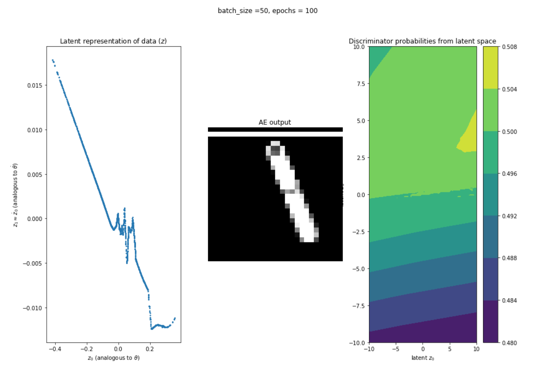
\includegraphics[width=\textwidth]{figures/gan_phase_1stack.png}
%\end{subfigure}
%\begin{subfigure}{0.7\textwidth}
%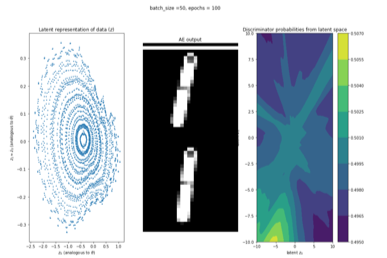
\includegraphics[width=\textwidth]{figures/gan_phase_2stack.png}
%\end{subfigure}
%\begin{subfigure}{0.7\textwidth}
%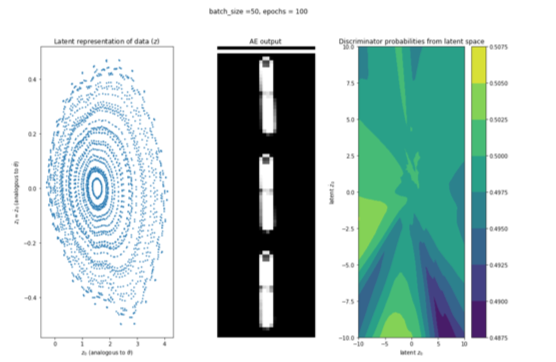
\includegraphics[width=\textwidth]{figures/gan_phase_3stack.png}
%\end{subfigure}
%\end{figure}
%
%We carried out an extensive study between batch size and epoch. However, we find no consistency in the generated phase space.
%
%\subsubsection*{key takeaways}
%
%Preliminary results show that GANs are difficult to work with (this could be an interesting topic to cover on its own). I believe gradient clipping is one way to solve this issue. 
%More importantly, Variational Integrator Networks proves that the learnt phase space from an AE will not, in general, represent the true phase space. In order to do this, one needs to encode the Lie group dynamics.
%Constrained GANs have already been looked at for generating consistent results.
%
%We still have yet to establish why a potential Lie group constrained GAN can help the world. i.e. why is it useful to be able to generate random samples of a pendulum swinging?
%
%
%\subsection{VIGN}
%
%Need to fill this section out in detail.
%
%
%\subsection{Lagrangian Dynamics (WIP)}
%The Euler-Lagrange formulation equates to:
%
%$$ \frac{\partial}{\partial t} (\frac{\partial L}{\partial \dot{q}}) = \frac{\partial L}{\partial q} $$
%
%where:
%$$ L = T - U $$
%
%In the example of a pendulum:
%
%$$ T = 1/2 mv^2 = 1/2 m (l\dot{\theta})^2 = 1/2 m l^2 \dot{\theta}^2 $$
%
%$$ U = mgh = mgl(1- \cos \theta) $$
%
%$$ L = 1/2 m l^2 \dot{\theta}^2 - mgl(1-\cos\theta) $$
%
%Placing the above into the euler-lagrange form gives us:
%
%LHS:
%
%$$ \frac{\partial L}{\partial \dot{q}} = ml^2 \dot{\theta}$$
%
%$$ \frac{\partial}{\partial t} (\frac{\partial L}{\partial \dot{q}}) = ml^2 \ddot{\theta} $$
%
%RHS:
%
%$$ \frac{\partial L}{\partial q} = -mgl\sin\theta$$
%
%Therefore:
%
%$$ \ddot{\theta} = \frac{g}{l} \sin \theta $$
%
%
%Now, to transition to the Hamiltonian version:
%
%We can write the hamiltonian as the sum of the energies:
%
%$$ H = T + U $$
%
%$$ H = p^2/2m + U $$
%
%$$ H = -L + 2K $$
%
%$$ H = -L + mv^2$$
%
%$$ H = -L + p^2/m = -L + p* (m\dot{q})/m = -L + p\dot{q}$$
%
%$$ p = \frac{\partial L}{\partial \dot{q}} $$
%
%
%\section{Running Ideas}
%
%\subsection{VIGN extension}
%
%- non conserved energy domain
%is there a link between the port-hamiltonian view and lagrangians with generalized force
%for a damped system we have:
%
%$$ \frac{d}{dt} \frac{\partial \mathcal{L}}{\partial \dot{q}} - \frac{\partial \mathcal{L}}{\partial q} = \mathbf{F}^{ext} \frac{\partial \mathbf{r}}{\partial q}$$
%
%see \href{http://www.physics.hmc.edu/~saeta/courses/p111/uploads/Y2013/lec131023-DSHO.pdf}{here} for details on how this equation was built. 
%
%- distributional assumptions for practical purposes
%
%Assume $ H = E_c $ for a trajectory of an initial condition, then:
%
%$$ H = K + U $$
%
%$$U = H - K $$
%
%$$ L = K - U $$
%
%$$ L = 2K -H $$
%
%Now, for L to be constant, K needs to be constant. In most cases, $ K = p^2/2m $. For this to be constant p should be constant. For p to be constant, $\dot{p} = 0$. This would imply, for most settings, that:
%
%$$ \frac{dp}{dt} = \frac{dU}{dq} = 0 $$
%
%This means that U is zero, which is not true.
%
%We have proven that as long as energy is conserved in a system exhibiting $K = p^2/2m$ the Lagrangian will never be constant unless the system has 0 potential. 
%
%As such, the Lagrangian depends on the distribution of the kinetic energy/potential energy. In the large N limit, these distributions tend toward a Gaussian.
%
%Is it beneficial to have a target variable distributed more broadly like a gaussian vs a delta?
%
%
%\subsection{Covid}
%
%
%SEIR model is differentiable and has some hamiltonian/energy conserving property. how might we build a neural network on this?
%
%We start out using SEIR to model china and it works well.
%
%We have issues modeling beijing which is seeing a second spike, we could reshape R naught (t) as an exponential sine function.
%$$ R_0(t) = Ae^{-(t-t_0)}|sin(B(t-t_0))| $$
%
%This is too specific. How can we encode the SEIR model into a graph neural network. Note, graph networks and graph neural networks are different frameworks encompassing the same core operations. In graph networks, however, the intermediate functional representations (hidden layers) are computed first, before an aggregation scheme is used. In graph neural networks, e.g. GCN, the operations involve computing a hidden layer first using neighbouring nodes, before feeding these hidden layers into the graph neural network.
%
%This reversal means one needs to be careful in how they define graph neural network architectures between DGL and deepmind graph nets library.
%
%We use graph convolutions to train on simulated data, we find hypersensitivity to initial conditions. More importantly, because of the time dependent nature of the system we are unsure of how many lag-variables are necessary to evolve the system.
%
%\subsection{Inductive  biases for RL}
%
%MDPs with policies which are deterministic or stochastic. Model free which involves sampling at random. Model based which involves sampling the learnt environment.

\pagebreak
\bibliography{references.bib}



\end{document}
